\section{Evaluation}
\label{sec:eval}

\sloppy{}
The evaluation answers the following research questions in order as follows. 

\begin{itemize}
\item What is the performance overhead of \cheetah{}? (\ref{sec:perf})

\item How effectively can \cheetah{} detect false sharing problems? How helpful are the outputs in fixing false sharing problems? (\ref{sec:effectiveness})

\item How is the precision of assessment on each false sharing instance? (\ref{sec:precision})

\end{itemize}

\paragraph{Experimental Setup.} We evaluate \cheetah{} on an AMD Opteron machine, which has 48 1.6 GHz cores, 64 KB private L1 data cache, 512 KB private L2 cache, 10 MB shared L3 cache, and 128 GB memory. We use gcc-4.6 with {\tt -O2} option to compile all applications. Since the machine is a NUMA machine and the performance may vary with different scheduling policies, we bind the threads to cores in order to acquire consistent performance.   

\paragraph{Evaluated Applications.} As prior work~\cite{Sheriff, Predator, qinzhao, mldetect}, we perform experiments on two well-known benchmark suites, Phoenix~\cite{phoenix-hpca} and PARSEC~\cite{parsec}. We intentionally use 16 threads in order to run applications sufficiently long, since \cheetah{} needs enough samples to detect false sharing problems.  Basically, we want to make every application run at least 5 seconds to collect enough samples. For PARSEC benchmarks, we are utilizing the \texttt{native} input. For some applications of \texttt{Phoenix}, we explicitly change the source code for \texttt{linear\_regression} by adding more loops. 

\subsection{Runtime Overhead}
\label{sec:perf}

\begin{figure*}[htbp]
\centering
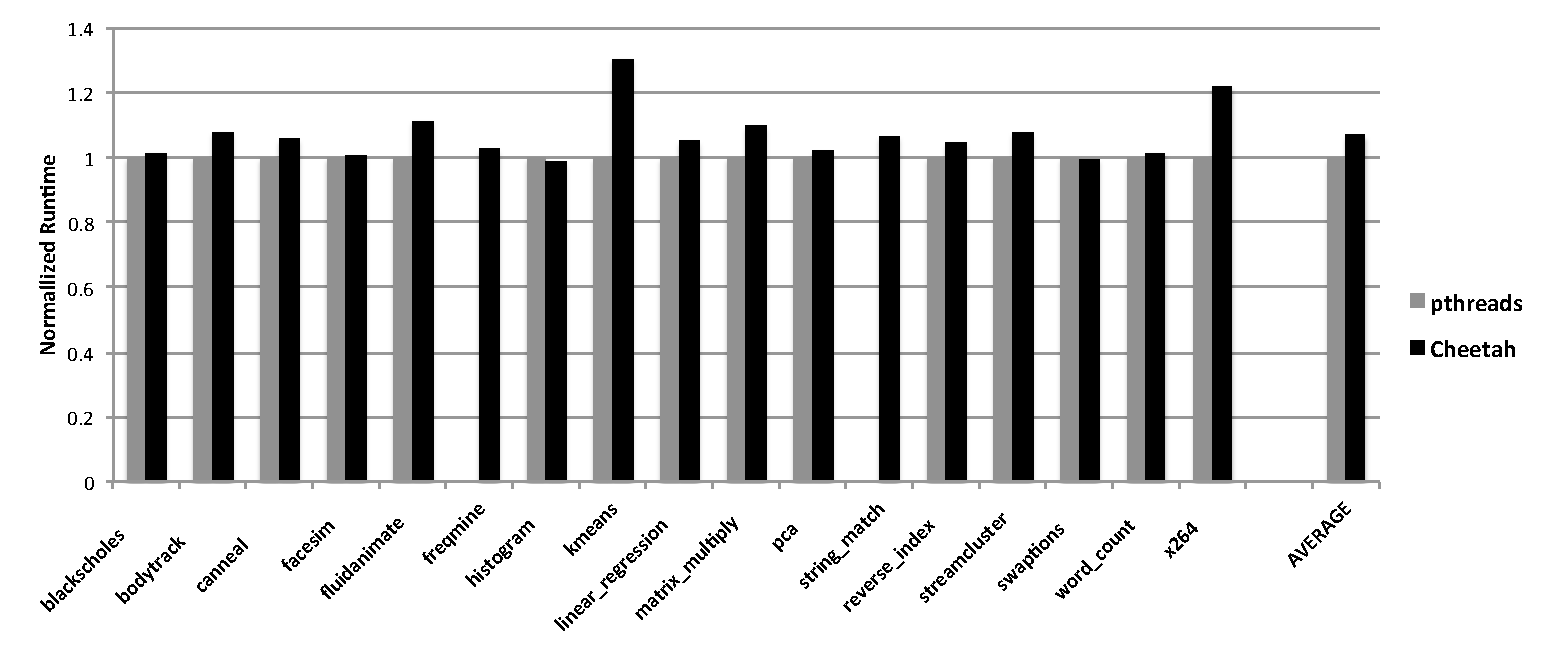
\includegraphics[width=2\columnwidth]{figure/Overhead.pdf}
\caption{Runtime overhead of \Cheetah{}. We normalize the runtime to that of native execution without monitored by \Cheetah{}. On average, \cheetah{} only introduces around 7\% performance overhead on all evaluated applications, which makes it practical to be used in real deployment. \label{fig:overhead}}
\end{figure*}

We show the average runtime overhead of \cheetah{} in Figure~\ref{fig:overhead}. We run each application for five times and show the average results here. According to this figure, \cheetah{} only introduces around 7\% performance overhead, which makes it practical to be utilized in the real deployment. 

During the evaluation, we configure \cheetah{} with the sampling frequency at one out of 64K instructions. Thus, for every 64K instructions, the signal handler is notified once and filters out instruction samples without memory access.
\cheetah{} can then associate memory access samples with heap and global variables. Currently, \Cheetah{} skips memory accesses in kernel, libraries or others. 

The performance overhead of \cheetah{} mainly comes from the handling of each sampled memory access and each thread creation. For each sampled access, we collect information, such as the type of access (read or write), the number of cycles, and update  the history table of its corresponding cache line. \cheetah{} also intercepts every thread creation to set up the PMU unit, get the timestamp and update the phase information. For applications with a large number of threads, including \texttt{kmeans} (with 224 threads in 14 seconds) and \texttt{x264} (with 1024 threads in 40 seconds), setting PMU registers introduces non-negligible overhead since it invokes six \texttt{pfmon} APIs and six additional system calls. For other applications, \cheetah{} introduces less than 12\% performance overhead, with 4\% overhead on average if these two applications are excluded.  

%\todo{Check the creation of threads for kmeans and x264. Initializing IBS registers for every thread adds significant performance overhead. Kmeans 224 threads in 14 seconds. 1023 threads in 40 seconds.  }

%\todo{Should we check how the performance overhead will be changed at a different sample frequency?}
 
\subsection{Effectiveness}
\label{sec:effectiveness}

%The state-of-the-art tool Predator reports five false sharing instances in Phoenix and Parsec benchmark suite, including \texttt{histogram}, \texttt{linear\_regression}, \texttt{reverse\_index}, \texttt{streamcluster}, and \texttt{word\_count}~\cite{Predator}. 
\cheetah{} successfully detects two known false sharing problems with significant performance impact, including\texttt{linear\_regression} in Phoenix and \texttt{streamcluster} in PARSEC. 

%In the remaining of this section, we discuss how reported information can help us to confirm and fix these false sharing problems. 

%Finally, we study the false sharing that \cheetah{} does not detect in these benchmarks and verify that they have negligible impact to the overall program execution. 

\subsubsection{Case Study: linear\_regression}
Figure~\ref{fig:lr} shows the output of \cheetah{}. It points out that the {\tt tid\_args} object allocated at line 139, with the structure type {\tt lreg\_args}, incurs a severe false sharing problem. According to the assessment, fixing it can possibly improve the performance by $5.7\times$. By examining the source code, we can discover that the {\tt tid\_args} object is passed to different threads --- linear\_regression\_pthread. Then we can easily find out where false sharing has been exercised, which is shown as Figure~\ref{lr:code}. By checking word-based accesses that are reported by \cheetah{} but not shown here, we can understand the reason of this false sharing problem: different threads are updating different parts of the object {\tt tid\_args} simultaneously, where each thread updates words with the size of the structure lreg\_args. This problem is similar to the example shown in Figure~\ref{fig:penalty}. 

To address the problem, we pad the structure {\tt lreg\_args} with extra bytes, by adding 64 bytes useless content, so that we can force different threads not to access the same cache line. The one-line code change leads to a 5.7$\times$ speedup of the performance, which matches the assessment of 5.76$\times$ improvement predicted by \cheetah{}.

\begin{figure}
\begin{minipage}{\columnwidth}

\centering

\fbox
{
%\scriptsize
\begin{minipage}{3in}
Detecting false sharing at the object: start 0x400004b8 end 0x400044b8 (with size 4000). \\
Accesses 1263 invalidations 27f writes 501 total latency 102988 cycles.\\
\\
Latency information: \\
totalThreads 16 \\
totalThreadsAccesses 12e1 \\
totalThreadsCycles 106389 \\
%longestRuntime 7652 \\
%threadReduceRate 0.164697 \\
totalPossibleImprovementRate 576.172748\% \\
(realRuntime 7738 predictedRuntime 1343).\\
\\
It is a heap object with the following callsite:\\
linear\_regression-pthread.c: 139
\end{minipage}
}
\vspace{1em}
\caption{\cheetah{} reports a false sharing problem in \texttt{linear\_regression}.}
\label{fig:lr}
\end{minipage}
\end{figure}


\begin{figure}
%\scriptsize
\begin{verbatim}
typedef struct
{
  ......  
  long long SX;
  long long SY;
  long long SXX;
  ......
} lreg_args;	

for (i = 0; i < args->num_elems; i++)
{
  //Compute SX, SY, SYY, SXX, SXY
  args->SX  += args->points[i].x;
  args->SXX += args->points[i].x
              *args->points[i].x;
  args->SY  += args->points[i].y;
  ......
}
\end{verbatim}
\caption{The data structure and source code related to a serious false sharing instance in \texttt{linear\_regression}.}
\label{lr:code}
\end{figure}

\subsubsection{Case Study: streamcluster}

%Figure~\ref{fig:sc} shows the output of StreamCluster. 
We do not show the report results of streamcluster because of space limit. For streamcluster, every thread will update the \texttt{work\_mem} object concurrently, allocated at line 985 of the \texttt{streamcluster.cpp} file. The authors have already added some padding to avoid false sharing. However, they assume the size of cache line (as a macro) to be 32 bytes, which is smaller than the size of actual cache line used in our experimental machine. Thus, streamcluster will still have a significant false sharing problem. The performance impact of fixing false sharing problems inside is further discussed in Section~\ref{sec:precision}. 


\subsubsection{Comparing with State-of-the-art}

\begin{figure}[htbp]
\centering
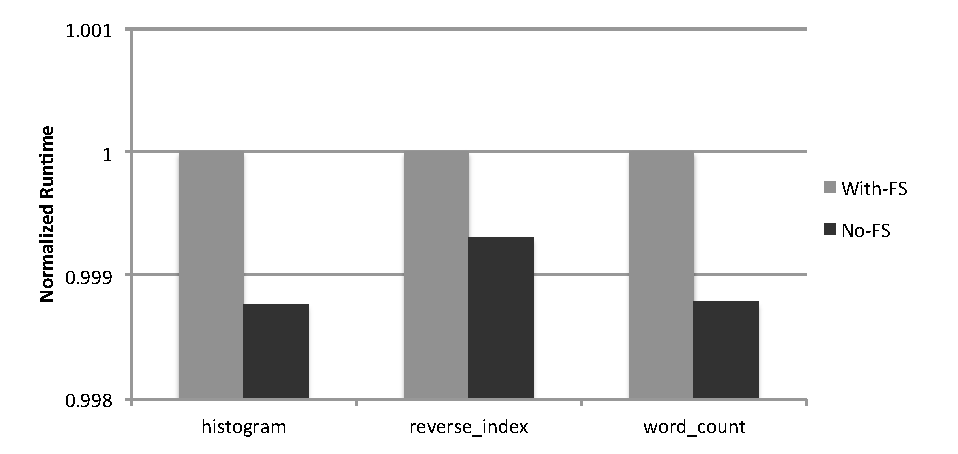
\includegraphics[width=1\columnwidth]{figure/trivial.pdf}
\caption{False sharing problems missed by \cheetah{} have negligible (<0.2\%) performance impact. \label{fig:fseffectiveness}}
\end{figure}

%\cheetah{} may miss some false sharing instances because of its sampling feature. 
Predator is the state-of-the-art in false sharing detection, which detects the most number of instances but with around $6\times$ performance overhead~\cite{Predator}. Comparing with Predator, \cheetah{} misses false sharing problems in \texttt{histogram}, \texttt{reverse\_index} and \texttt{word\_count}~\cite{Predator}. 

As discussed before, \cheetah{} only detects actual false sharing problems that may have significant performance impact on the final performance. If the number of accesses on a falsely-shared object is not large enough, \cheetah{} may not be able to detect it because of its sampling feature.  Also, the occurrences of false sharing can be affected by the starting address of objects or the size of the cache line or be affected by the cache hierarchy, as observed by Predator~\cite{Predator}. Thus, we further check the seriousness of these problems based on Predator's detection results. 

We run these applications on our experimental hardware, with and without false sharing problems. Figure~\ref{fig:fseffectiveness} shows the performance impact. Actually, these benchmarks do not show a significant speedup after fixing, with less than 0.2\% performance improvement. This behavior actually exemplifies the advantage of \Cheetah{}: since \cheetah{} only reports false sharing problems with significant performance impact, it can potentially save programmers manual effort unnecessarily spending on applications with trivial performance improvement. 

\subsection{Assessment Precision}
\label{sec:precision}

\cheetah{} is the first tool that can assess the performance impact of false sharing problems. Based on this information, programmers may save huge amount of manual effort spending unnecessarily on applications with trivial false sharing problems. 

We evaluate the precision of assessment on two applications that are detected to have false sharing problems, \texttt{linear\_regression} and \texttt{streamcluster}. We list the precision results in Table~\ref{tbl: precision}. In this table, \texttt{linear\_regression} is abbreviated as ``\texttt{linear\_reg}''.  We evaluate these applications when the number of threads is equal to 16, 8, 4, and 2 correspondingly. We list the predicted performance impact in the ``Predict'' column and the actual improvement in the ``Real'' column of the table. The last column (``Diff'') of this table lists the difference between the predicted improvement and the real improvement. If the number is larger than 0, the predicted performance improvement is less than the real improvement. Otherwise, it is the opposite. 
%The difference is calculated by dividing the difference by the real improvement.  

Table~\ref{tbl: precision} shows that \cheetah{} can perfectly assess the performance impact of false sharing in every case, with less than 10\% difference for every evaluated execution. %Relying on the assessment, programmers do not have to spend time on trivial false sharing problems any more. 
%\emph{According to this novel assessment of \cheetah{}, programmers may save huge amount of manual effort spending unnecessarily on applications with trivial false sharing problems}. 

\begin{table}
  \small
  \centering
  \begin{tabular}{ c | c | c | c | c}
  \hline
  \textbf{Application} & \specialcell{Threads \\ (\#)} & \textbf{Predict} & \textbf{Real} & \specialcell{Diff \\ (\%)}\\ \hline
\texttt{linear\_reg} & 16 & 6.44X    & 6.7X & {-3.8}\\
\texttt{linear\_reg}& 8  & 5.56X    & 5.4X & {+3.0}\\
\texttt{linear\_reg} & 4  & 3.86X  & 4.1X  & {-5.8}\\
 \texttt{linear\_reg}& 2  & 2.18X  & 2X    & {+9}\\ \hline
 \texttt{streamcluster} & 16 & 1.016X    & 1.015X &  {0}\\
 \texttt{streamcluster} & 8 & 1.017X    & 1.018X & {0}\\
 \texttt{streamcluster} & 4 & 1.024X    & 1.022X & {0}\\
 \texttt{streamcluster} & 2 & 1.033X    & 1.035X & {0}
 %\hline
\end{tabular}
  \caption{
    Precision of assessment. \Cheetah{} implements the first method to accurately predict the performance improvement of fixing an observed false sharing instance. \label{tbl: precision}}
\end{table}

